\chapter{Outlook} \label{ch:outlook}
While \glspl{carb} will provide a considerable performance advantage for larger quantum computers in the NISQ era, their up-scaling to larger systems also entail new challenges and open questions.

A first challenge relates to the elaborate \gls{carb} calibration procedure, although a few straight-forward improvements are expected to increase the calibration speed by an order of magnitude (see Section~\ref{sec:carb_calibration}). While we implemented the gate for fixed-coupling,  frequency-tunable transmons using unipolar flux pulses, other gate architectures might provide a higher level of convenience. One promising approach is a gate based on a tunable $ZZ$-coupling achieved with a frequency tunable coupler qubit \cite{Collodo2020}.  Independently of the flux pulse parametrization, this gate acquires conditional phase linearly as function of interaction time which eases the calibration and potentially reduces interpolation errors. In addition, the acquired dynamic phase changes slowly as a function of other gate parameters, which reduces the number of calibration points and therefore the overall tune-up time of the gate. 

Developing rapid and adequate characterization techniques for continuously parametrized gates designed for \glspl{vqa} is a second aspect arising from this thesis, and is not clearly established in literature. Although quantum process tomography provides full information about the quantum process, it also suffers from leakage, preparation errors and does not offer an intuitive interpretation for the different error sources. 

Inspired from Ref.~\cite{Abrams2019ImplementationPulse}, we propose an alternative characterization method for benchmark pairs of subsequent gates, with conditional phases of $\pi-\alpha$ and $\alpha$ respectively. Since the conditional phase of these two gates sums up to $\pi$, the combination of the two gates corresponds to a \gls{cz} which is in the Clifford group.  Randomized benchmarking therefore allows to put a bound on the error of the combination of two gates (but not on the individual gates). Cross-entropy benchmarking \cite{BarendsDiabaticQubits} is another approach that can assess the performance of non-Clifford gates and has been used by Ref.~\cite{Foxen2020DemonstratingAlgorithms} for their continuously parametrized gates.

However, both randomized and cross-entropy benchmarking are insensitive to small coherent errors which can accumulate quickly and cause deleterious effects in algorithms with repetitive structures (such as \gls{qaoa}) \cite{Kjaergaard2020AProcessor}. A recent calibration method based on quantum process tomography of long strings of CZ gates alleviate these effects \cite{Kjaergaard2020AProcessor} and could be extended to \glspl{carb}.

As we progress towards larger experiments, we will have the opportunity to explore more complex problem instances. In Fig.~\ref{fig:outlook_problem_instances}(b) and (c), we present two exact cover problem instances designed for the device described in Ref.~\cite{Andersen2019RepeatedCode}, whose hardware connectivity graph is reproduced in Fig.~\ref{fig:outlook_problem_instances}(a). The former instance respects the connectivity of the device and has two solutions, $\mathcal{L}_1 = \{A, D, G\}$ and  $\mathcal{L}_2 = \{B, C, E, F\}$. By contrast, the latter instance represents a dense problem graph that require interactions between qubits which are not physically connected and has a single answer, $\mathcal{L} = \{C, E, F\}$. The implementation thereof requires SWAP-gates which lengthen the gate sequence for each \gls{qaoa} layer. While the SWAP-gates themselves can be decomposed into \glspl{cz} and single qubit gates, the sequence would be much shorter if the SWAP operations are part of the available hardware gate set. Due to the higher problem graph connectivity and the uniqueness of the solution, the number of layers required to find a good approximate solution is higher for the second problem instance. 

\begin{figure}[ht]
    \centering
    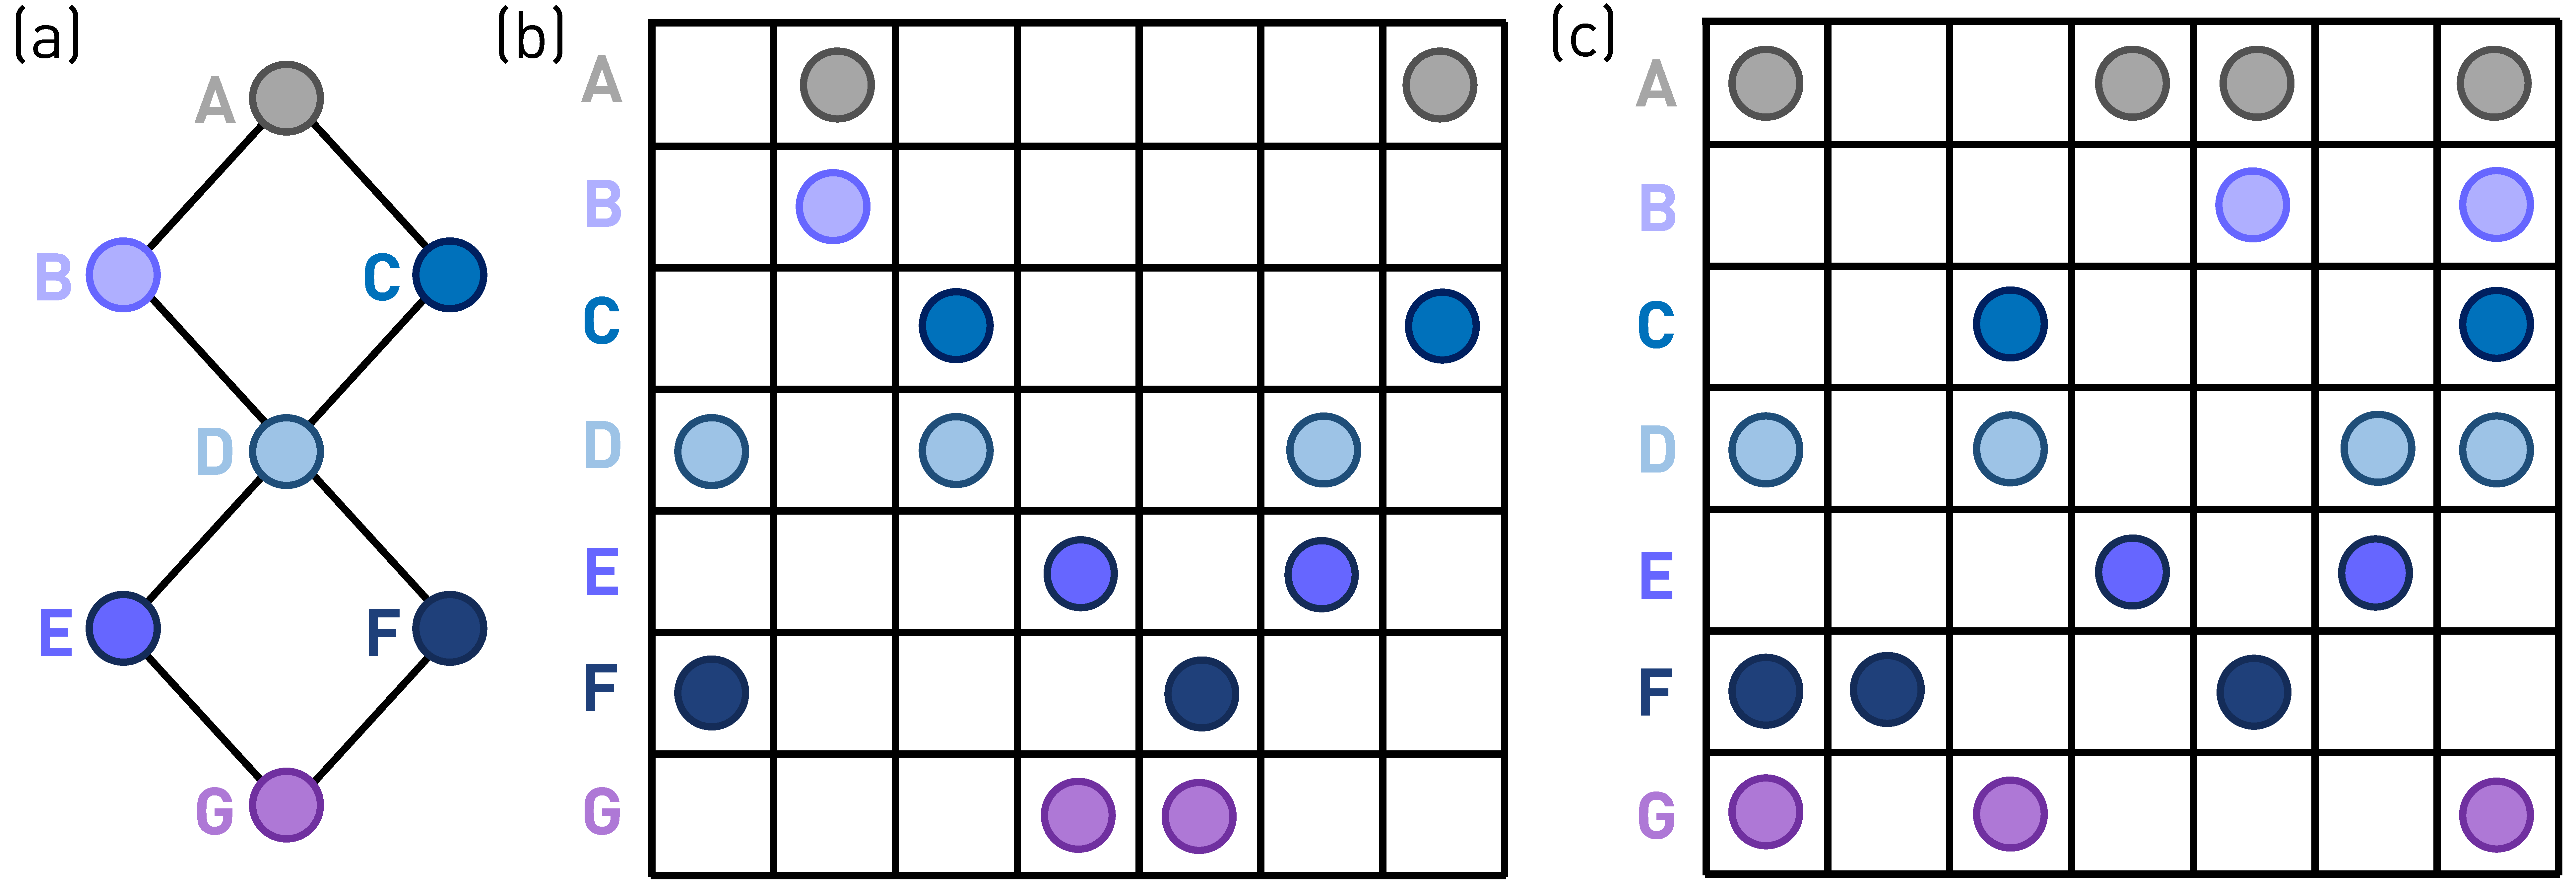
\includegraphics[width=\textwidth]{outlook_problem_s7.pdf}
    \caption{Example of future experiments designed for a 7-qubit quantum processor. (a) Hardware graph connectivity of the 7-qubit quantum processor described in Ref.~\cite{Andersen2019RepeatedCode}. (b) Incidence matrix of an exact cover problem instance respecting the connectivity of (a). (c) Incidence matrix of an exact cover problem instance requiring full "logical" connectivity and therefore SWAP operations between the physical qubits. }
    \label{fig:outlook_problem_instances}
\end{figure}

Finally, the use of the \gls{carb} is foreseen to extend beyond \gls{qaoa}, with potential applications in quantum chemistry~\cite{Jiang2018QuantumFermions} and quantum neural networks~\cite{Cao2017QuantumComputers}.